\chapter{Fundamentals}\label{chap:fundamentals}

In this chapter, first the basics of localization are introduced. Afterwards, the \acf{PF} and \acf{MCL} algorithm are explained. The detailed reasons for choosing \ac{MCL} for the solution are pointed out in Section~\ref{sec:algo_decision}. At the chapter's end, an overview of further localization approaches used in related work, is given.

\section{Fundamental Aspects of Localization}\label{sec:fund_loc}

Localization, i.e.\ positioning, is the process of estimating the position of an object in its environment. Usually the object's environment is defined by using a coordinate system. One of the most popular coordinate systems is the \emph{World Geodetic System 1984 (WGS84)}, which describes a position on earth, by longitude and latitude. Sometimes, it is sufficient to use a local coordinate system; for instance, a two or three dimensional cartesian coordinate system. Indoor localization is one example, where it is sufficient to use a local coordinate system, because the object's position is limited to a defined area, e.g.\ within a building.

\subsection{Location Types}
There are four types of locations. A \emph{physical location} is described by coordinates on a map. \emph{Symbolic locations} such as ``in the living room'' or ``on the small table in the kitchen'', are often used by humans. If all objects share a frame of reference, like chess pieces on a chess board, the type of location is called an \emph{absolute location}. When an object has its own reference frame, as for instance when saying ``I am two meters away from the door'', which often includes a proximity value, it is called a \emph{relative location} \citep{IEEE:survey_wireless_indoor_pos}.

Typically indoor localization is based on absolute locations, because all objects, such as landmarks, obstacles (i.e.\ occupied space), and corridors (i.e.\ free space) share the same frame of reference, i.e.\ the building's map. It is also possible to use physical locations for indoor positioning by either transforming the objects' absolute positions into physical positions or by knowing them. In the following a location is usually an absolute location.

\subsection{System Topology}
Usually, a pure wireless localization system consists of at least one transmitter that emits some sort of signal, and one or more receivers, i.e.\ measuring units. The system's topology can be \emph{remote positioning}, which means that the transmitter's position is estimated by using the measurements from multiple measuring units, that are deployed at fixed locations. The position estimation takes place in a component separate from the transmitter. This component uses the measurements as input. If the measurement unit is mobile and capable to estimate its own position by collecting the signals from fixed transmitters, the system's topology is called \emph{self-positioning}. \emph{Indirect remote positioning} is basically the same as self-positioning, but the collected measurements are sent via some data connection to an external service, which performs the position estimation. If the system's topology is basically remote positioning, but the measurements are transferred via a wireless data link to the mobile side, the topology is called \emph{indirect self-positioning} \citep{IEEE:survey_wireless_indoor_pos}.

Besides a pure wireless localization systems, which just uses wireless signals for the positioning, other systems, often used in the area of mobile robotics, do exist. Robots are often equipped with sensors, such as laser scanners or ultrasonic sensors, to measure distances to obstacles. Wheel- and chain-based robots are usually also equipped with odometers, others have accelerometers and rotation rate sensors to estimate the traveled distance. The used localization algorithms are able to combine different sensors to provide a more accurate estimation \citep{thrun:prob_robo}. Mobile robots, especially if they operate autonomously, are usually self-positioning, or indirect remote positioning systems, which often depends on their system's hardware capabilities. Remote positioning as well as indirect self-positioning systems are rarely the case in the field of mobile robots.

The presented solution is a self-positioning system. It measures the distances to known beacons, but it not only relies on the measured wireless signals, it uses also the user's motion like a robot. Thus, the user's smartphone is the mobile measuring unit, which additionally does the whole position estimation.

\subsection{Uncertainty}
In order to derive an accurate position, localization systems need to be able to accommodate uncertainty. According to \citet{thrun:prob_robo}, uncertainty in robotic systems has several reasons.

One of these reasons is the \emph{environment}. If a robot works together with humans, the environment is very dynamic and unpredictable, because the robot does not know for; instance, where and when a human moves to.
Of course, robots are equipped with \emph{sensors} to recognize obstacles like humans, but sensors may also cause uncertainty. On one hand, they have limitations, e.g.\ a camera has a specific resolution, and on the other hand, noise may unpredictably influences their measurements. 
Typically, robots have \emph{actuators}; for instance, motors to move them within their environment. Actuators have precision limitations. Additionally, their successive physical components; for instance, a robot's wheels on different surfaces, may cause unpredictable effects.
To allow robots to operate in a physical environment, models of it are used. \emph{Models} are abstractions, which approximate a certain object or behavior. Thus, information is lost, and additionally every model contains some inaccuracy. Robotic systems work in real-time environments. Due to computational reasons, their \emph{algorithms} cannot really operate in real-time. In reality, a physical property changes continuously, but a robot's measurements can only be processed in certain time steps, which causes inaccuracy. 

All mentioned factors together might cause large uncertainty. Thus, the system needs to be able to accommodate or somehow compensate for it. This is the reason, why the algorithm, introduced in Chapter~\ref{chap:pf}, not only relies on the distance measurements to the beacons. Due to the uncertaintys' high importance, the used sensors' uncertainty is discussed at the end of Chapter~\ref{chap:ibeacons} and \ref{chap:sensors}.

\subsection{Localization Problems}
Localization is not always the same. There are different localization problems depending on the environment and the use-case of the application. According to \citet{thrun:prob_robo} the following problems exist:
\begin{itemize}
\item \textbf{Local vs.\ Global Localization:} If the initial position is known when the localization starts, a so-called position tracking only is necessary, to know future positions. This is called \emph{local localization}. In the case where the initial position is unknown, and this position can by anywhere on the map, this is called \emph{global localization}. These types of algorithms are more difficult than position tracking. Global localization solves also the \emph{kidnapping} problem, which means that e.g.\ a robot is being placed on a different position during the position estimation. Of course, that is not very typically, but by solving this problem the algorithm is also able to recover if it is stuck in a state where it never will be able to approximate the true position.

\item\textbf{Static vs.\ Dynamic Environments:} In a \emph{static environment} the localizing object, e.g.\ a robot, is the only object that changes its position over time. All obstacles and other objects maintain their fixed position. In a \emph{dynamic environment} other objects besides the localizing object can change their position. Typical objects in a dynamic environment are humans, furnitures, like chairs or doors that sometimes are moved, closed or opened.

\item\textbf{Passive vs.\ Active Approaches:} If the localization algorithm is able to control the localizing object's motion, this is called an \emph{active approach}. Through the ability to influence a motion, the algorithm can induce movement of the object, e.g.\ the robot, if the localization is stuck and needs more information; for example, from another point within a room, to decide what its position is. \emph{Passive} algorithms just observe the motion, but cannot influence it. Usually, active approaches are built upon passive ones.

\item\textbf{Single-Robot vs.\ Multi-Robot localization:} \emph{Single-Robot} localization means, that the robot only needs to localize itself. \emph{Multi-Robot} localization requires of course multiple robots in the same area. It builds upon single-robot localization; thus, each robot can estimate its own position. New opportunities arise if the robots can recognize, each other and are able to communicate, to exchange their estimated positions.
\end{itemize}

\noindent The solution presented in this thesis, solves the global localization and kidnapping problem in a dynamic environment; whereas, the in Chapter~\ref{chap:evaluation} presented results where measured in a static environment. The algorithms implementation is a passive approach. Furthermore, the solution only solves the Single-``Robot'' localization problem, but Chapter~\ref{chap:conclusion} presents an idea how Multi-``Robot'' localization could be used to improve the presented solution.

\subsection{Performance Metrics}
To be able to compare different localization systems and algorithms the following criteria, recommended by \citet{IEEE:survey_wireless_indoor_pos}, is introduced. Often the system's accuracy is the only metric being used. But also from my opinion as well, the system's accuracy is not sufficient for evaluation purposes. In addition to the metrics recommended by \citet{IEEE:survey_wireless_indoor_pos}, the system's usability is in my opinion another important criteria.
\begin{itemize}
	\item \textbf{Accuracy} is the error of the estimated position. It is the Euclidean distance between the estimated and the real position.
	\item \textbf{Precision} takes the consistency into account. \citet{IEEE:survey_wireless_indoor_pos} defines it as the result of ``the cumulative probability function[s] (\acs{CDF}) of the distance error'', for instance 90\,\% location precision within 2\,m, i.e.\ \acs{CDF}(2\,m)\,=\,0.9.
	\item \textbf{Complexity} depends on several factors, such as the required hardware, the software complexity, the algorithms complexity, the necessary infrastructure, etc. However, \citet{IEEE:survey_wireless_indoor_pos} focus on software, i.e.\ computing complexity only.
	\item \textbf{Robustness} expresses the ability of a system to deal with wrong sensor data, unexpected values, or even no sensor data within a certain time interval.
	\item \textbf{Scalability} describes the possibility of a system to be extended or reduced in space, or a change of the density of the transmitters or measurement units.
	\item \textbf{Cost} depends on several factors. The financial costs are a very important factor. This depends on the hardware, implementation and installation costs. The energy consumption, which in the end also reflects in financial cost, is also an important factor. The factor time is also not negligible. The amount of time it takes to deploy and maintain such a system can be enormous.
	\item \textbf{Usability} depends mainly on the system's user friendliness, i.e.\ is it difficult for the user to use the system, is the system self-explaining, etc. If a system's usability is very bad its usually not being accepted by the users.
\end{itemize}

\noindent In Chapter~\ref{chap:evaluation}, the presented solution is evaluated against these criterias, with focus on the system's accuracy and precision.


\section{Particle Filter Algorithm and Related Work}\label{sec:fund_pf}
The solution presented in this thesis builds upon \acf{MCL}, which is based on \acf{PF}. This section introduces first the \ac{PF}'s basics and afterwards the fundamentals of \ac{MCL}. Finally, it gives an overview of related work, based on \ac{PF} and \ac{MCL}.

\subsection{Introduction to \acl{PF}}
The \ac{PF} is a non-parametric filter, i.e.\ it does not have fixed parameters which describe its distribution's functional form. By contrast \acf{KF} is a parametric filter, which parameters describe its functional form, i.e.\ a Gaussian distribution. \ac{PF} approximates the functional form by a finite number of values, often referred to as \emph{particles} or \emph{samples}. The approximation's quality depends on the particle set's size. Figure~\ref{fig:pf_approx} illustrates the approximation of a posterior distribution by samples. It also shows, that \ac{PF} is well-suited for multi-modal distributions \citep{thrun:prob_robo}.

\begin{figure}
	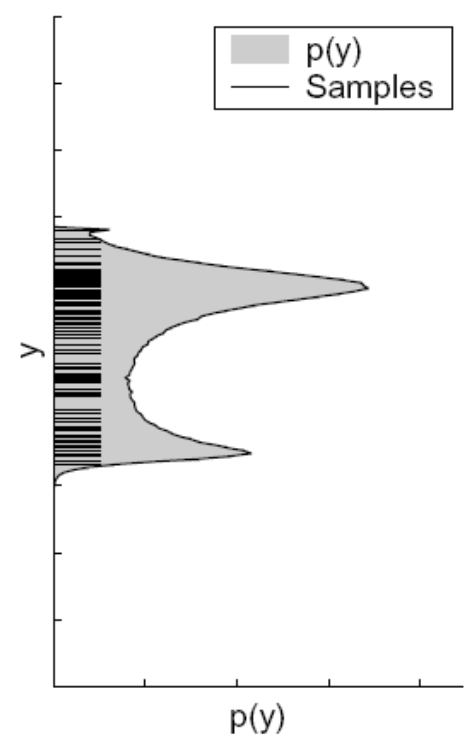
\includegraphics[height=0.45\textwidth]{figures/pf_approx}
	\caption{Approximation of a random variable Y, i.e.\ a posterior distribution by samples \citep[p.97]{thrun:prob_robo}.}
	\label{fig:pf_approx}
\end{figure} 

\begin{lstlisting}[
  float,
  floatplacement=H,
  mathescape,
  captionpos=b,
  caption=Algorithm for \acl{PF} based on \citet{thrun:prob_robo},
  label=lst:pf]
ParticleFilter($\chi_{t-1}$, $u_t$, $z_t$) {

  $\bar{\chi}_t = \emptyset$
  for $m = 1$ to $M$ {
    sample $x^{[m]}_t \sim p(x_t|u_t, x^{[m]}_{t-1})$
    $w^{[m]}_t = p(z_t|x^{[m]}_t)$
    add $\langle x^{[m]}_t, w^{[m]}_t \rangle$ to $\bar{\chi}_t$
  }


  \\ resampling
  $\chi_t = \emptyset$
  while size of $\chi_t$ less $M$ {
    draw $i$ with probability $\propto w^{[m]}_t$
    add $x^{[i]}_t$ to $\chi_t$
  }

  return $\chi_t$
}
\end{lstlisting}
 % label= lst:pf

According to \citet{thrun:prob_robo}, the idea is the posterior's~$bel(x_t)$ representation by a random set of samples, drawn from the posterior. Each sample~$x$ at time~$t$ is a hypothetical state in state space, i.e.\ in real world. The particle set $\chi_t = \left\{ x^{[1]}_t, x^{[2]}_t, \ldots, x^{[M]}_t \right\}$ is the distribution's approximation, containing $M$~particles. The \ac{PF}'s algorithm, depicted in Listing~\ref{lst:pf}, transforms the posterior~$bel(x_{t-1})$, represented by the particle set~$\chi_{t-1}$, by integrating the latest control~$u_t$ and measurement~$z_t$ into the current posterior~$bel(x_t)$. Thus, the algorithm creates first an empty, temporary particle set~$\bar{\chi}_t$. Then, the states from $\chi_{t-1}$ are updated by integrating the current control~$u_t$. Formally, this is done by sampling the new state~$x^{[m]}_t$ from the \emph{state transition probability}~$p(x_t|u_t, x^{[m]}_{t-1})$ (Listing~\ref{lst:pf}, Line 5). Afterwards, an \emph{importance factor}~$w^{[m]}_t$ for the new sample~$x^{[m]}_t$ is calculated (Listing~\ref{lst:pf}, Line 6). It is defined as $p(z_t|x^{[m]}_t)$, which is the probability for the measurement~$z_t$ given the new state hypothesis, representing a value in real world. The new state hypothesis and its importance factor are stored together as tuple, in the temporary set~$\bar{\chi}_t$ (Listing~\ref{lst:pf}, Line 7). The weighted set approximates the posterior~$bel(x_t)$.

Then, the resampling, i.e.\ importance sampling, transforms the weighted particle set, based on the particls' weights into a new set, which represents the new distribution. To do so, $M$~particles are drawn according their weight and inserted into the new set~$\chi_t$ (Listing~\ref{lst:pf}, Line 14, 15). During this step some particles are duplicated, usually the ones with high weight, and others, the ones with low weight, are lost. \citet{thrun:prob_robo} compares it with the Darwinian idea of \emph{survival of the fittest}. According to them, ``it refocuses the particle set to regions in state space with high posterior probability''.
 
Instead of the drawing, it is also possible to have a weighted set~$\chi_t$. In every recursion, the weights of the existing particles are multiplied with their new weight. The method's disadvantage is, that a larger particle set is required to reach the same approximation quality, because the particles keep their position in state space for ever, i.e.\ the particle cloud does not move. For this method the particle weight~$w^{[m]}_t$ of each particle needs to be initialized with 1.
 
\ac{PF} can be adaptive; for instance, based on the available processing power. The particle set is then being increased or decreased to adapt to the available processing power \citep{thrun:prob_robo}.


\subsection{Monte Carlo Localization}\label{sec:fund_mcl}
\ac{MCL} is a popular localization algorithm often used in the indoor mobile robotics field. The algorithm can deal with a broad range of the before discussed localization problems, especially with the local and global localization problem.

\begin{lstlisting}[
  float,
  floatplacement=H,
  mathescape,
  captionpos=b,
  caption=Basic \acl{MCL} algorithm based on \citet{thrun:prob_robo},
  label=lst:mcl]
mcl($\chi_{t-1}$, $u_t$, $z_t$, map) {

  $\bar{\chi}_t = \emptyset$
  for $m = 1$ to $M$ {
    $x^{[m]}_t$ = sample_motion_model($u_t$, $x^{[m]}_{t-1}$)
    $w^{[m]}_t$ = measurement_model($z_t$,$x^{[m]}_t$, map)
    add $\langle x^{[m]}_t, w^{[m]}_t \rangle$ to $\bar{\chi}_t$
  }


  \\ resampling
  $\chi_t = \emptyset$
  while size of $\chi_t$ less $M$ {
    draw $i$ with probability $\propto w^{[m]}_t$
    add $x^{[i]}_t$ to $\chi_t$
  }

  return $\chi_t$
}
\end{lstlisting}


The basic algorithm, shown in Listing~\ref{lst:mcl}, is very similar to the \ac{PF}, presented in Listing~\ref{lst:pf}. The sampling from the \emph{state transition probability} is substituted by a method called \texttt{sample\_motion\_model}, which samples the new hypothesis by integrating the control~$u_t$ with respect to the motion and its uncertainties during the execution (Listing~\ref{lst:mcl}, Line 5). Furthermore, the \emph{importance factor} calculation is substituted by the \texttt{measurement\_model} function, which depends on the used sensor (Listing~\ref{lst:mcl}, Line 6). It uses the sensor measurements and their uncertainty to calculate the particles' importance factors. It additionally takes the environment's map into account. Usually, the map is used to calculate the importance factor based on the measurement~$z_t$; for instance, the distance to a landmark, where the landmark's position is stored in the map. But a map can also be used to detect particles at impossible positions, and thus to reduce their importance factor. A very detailed description of \ac{MCL} and variations of the algorithm is provided by \citet{thrun:prob_robo}.

\begin{figure}[width=0.9\textwidth, height=0.4\textheight]
	\subfloat[]{
  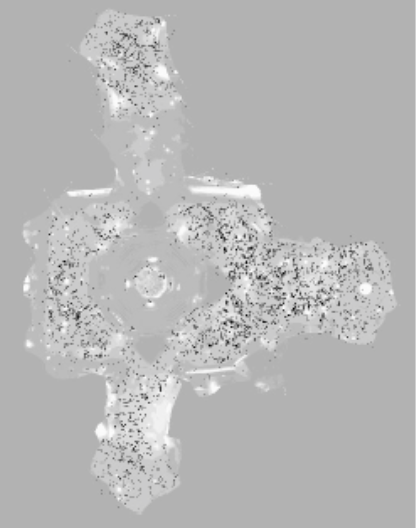
\includegraphics[width=0.3\textwidth]{figures/mcl_1}
}
\subfloat[]{
  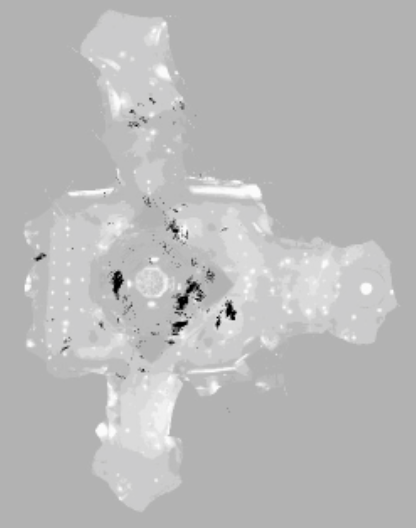
\includegraphics[width=0.3\textwidth]{figures/mcl_2}
}
\subfloat[]{
  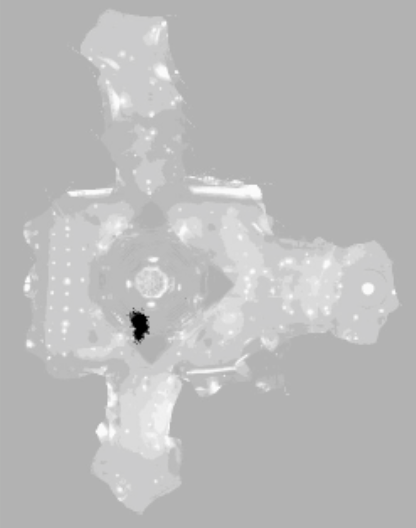
\includegraphics[width=0.3\textwidth]{figures/mcl_3}
}

	\caption{A visual example of the \acl{MCL} algorithm. It shows a building's map and the particle distribution over time \citep{thrun:prob_robo}.}
	\label{fig:mcl}
\end{figure}

A visual example of, how a global localization using \ac{MCL} works, is shown in Figure~\ref{fig:mcl}. The three images show the particles, i.e.\ the posterior $bel(x_k)$, over time. At the beginning uniform random particles are distributed over the whole state space, because the robot actually does not know where it is, and thus could be positioned anywhere. After moving and gathering sensor data, the particles concentrate in certain regions with higher probability for the true position. Thus, the posterior changes. In the end, the particles are concentrated on one spot; hence, the confidence of being at this position is very high \citep{thrun:prob_robo}.


\subsection{Related Work}

\citet{Siddiqui:tracking} proposes a localization system that uses \ac{PF} and \acs{RSS}-based trilateration of WiFi signals (explained in Section~\ref{sec:fund_trilateration}), to track a mobile unit. The approach relies solely on sensing \ac{RSS} values, no other sensors are used. First, they collect the \ac{RSS} values in their environment. They are stored together with their location in a lookup table. For their MATLAB simulation they generate a random path with 100~points using the before collected values. The path is tracked during the simulation, just based on the \ac{RSS} values. Their simulation simulates a notebook equipped with WiFi, which is tracked. Thus, their \ac{PF}'s implementation does not sample a new state by integrating the control~$u_t$ as mentioned before (Listing~\ref{lst:pf}, Line~5). They use two different weighting functions during their experiment, firstly, a \emph{Gaussian weighting function}, based on the Euclidian distance, and secondly, a \emph{Triangular weighting function} (Listing~\ref{lst:pf}, Line 6). According to \citet{Siddiqui:tracking}, their solution achieves an accurate localization of $\approx$\,3\,m as a result of their simulation. During the simulation they assume a static environment with sparse activity and a smooth and continuous motion. They also assume that no large variations in the signals' strength occur over short distances. In addition, they remove the first and last 10\,\% of the recorded measurements, i.e.\ when the person placed the measuring unit and picked it up again, to have independent values of a human in proximity. Additionally, they neglect outliers.

\citet{straub:pf} implementes an indoor pedestrian localization and tracking system based on \ac{PF}, which uses a system called \emph{PiNav}, developed at the institute where Straub wrote his thesis. It extracts the person's motion in form of step frequency, step size, and heading. The person needs to be equipped with the hip-mounted PiNav-System, which includes an accelerometer, gyroscope and a compass. Additionally, \citet{straub:pf} uses an accessibility map, which is based on a Neural Network, to learn which space on the map is accessible by pedestrians. By fusing the pedestrian's motion and the accessibility map in a \ac{PF}, his solution achieves an average accuracy of 1.1\,m \citep{straub:pf}.

\citet{wang:wlan} propose a \ac{RSS}-based WiFi positioning system using \ac{PF} to fuse the location estimated via WiFi with additional map and accelerometer data. Their system uses the in Section~\ref{sec:fund_sceneanalysis} mentioned Scene Analysis approach, especially the k-Nearest Neighbors~(kNN) algorithm for the positioning. During the offline stage they collect fingerprints of WiFi signals in one meter distance to the access points. During the localization, i.e.\ the online stage, the algorithm compares the fingerprints of the collected WiFi signals with the stored ones from the offline stage and returns a location estimation. According to \citet{wang:wlan}, the 3-axis accelerometer's values can be used in theory, to estimate the traveled distance by integrating the values. But, due to the low signal and the sensors' noise it does not work in praxis. Thus, they use a zero-crossing approach to detect steps and estimate their size. The approach detects a step if the vertical acceleration crosses the zero-line. Additionally, their solution uses the environment's map to sort out impossible particles, like particles crossing a wall.
Their simulation's results show, that by using map and accelerometer in addition to kNN, their location error improves by 40\,\%. Their solution is also 30\,\% better than the \ac{KF}'s result. During their real world tests, they achieved a mean error of 4.3\,m with a standard deviation of 2.8\,m \citep{wang:wlan}.

\citet{siddiqi:experiments_mcl_wifi} uses \ac{MCL} to globally localize a \emph{Pioneer 2DX} robot in an indoor environment using the robots odometers and the measured \ac{RSS} of WiFi signals. The algorithm's action model, i.e.\ motion model, is based on the data measured by the odometers. They deliver data for short distances with a very good accuracy. The motion is divided into translations and rotations. Their action model samples the motion with different uncertainties for translation and rotation. The observation model, i.e.\ measurement model, uses a signal strength map, which is divided into a grid with squared fields with a size of 0.5m. Before localization can take place, the \ac{RSS} of each WiFi access point for each grid cell needs to be measured to store \ac{RSS} mean and standard deviation for each cell. Due to the fact, that \citet{siddiqi:experiments_mcl_wifi} assume that the signal attenuation does not change on short distances, they just measure it for a few cells and assume the same value for the neighbor cells. During the localization, the actual \ac{RSS} values are compared with the collected values for the importance factor. Additionally, their observation model sorts out particles, by using the map constraints, but without taking the robot's orientation into account. According to \citet{siddiqi:experiments_mcl_wifi}, just using the map constraints without the \ac{RSS} comparison, already enables very good localization results.
During their tests they found out, that by increasing the amount of access points, the location error decreases \citep{siddiqi:experiments_mcl_wifi}. They mention, that their approach should also work for localization of humans instead of robots. But they also note, that a robot's motion model is simpler than the one of a human. According to \citet{siddiqi:experiments_mcl_wifi}, they achieve during most test cases an accurate localization with an error of $\approx$\,2\,m.


\section{Further Localization Algorithms and Related Work}
This section focuses on further localization algorithms, which are suitable for indoor self-localization using smartphones. Some algorithms are discussed in more detail than others, depending on their closeness to the solution presented in this thesis. After introducing the algorithm itself, an overview of related work, based on that algorithm, is given.

\subsection{Triangulation}\label{sec:fund_trilateration}
Triangulation is a well-studied localization method which relies on triangle's geometric properties \citep{IEEE:survey_wireless_indoor_pos, wang:bt_pos}. Triangulation is the hypernym of the two characteristics \emph{lateration} and \emph{angulation}.

\begin{figure}[width=0.9\textwidth, height=0.4\textheight]
	\subfloat[Lateration]{
  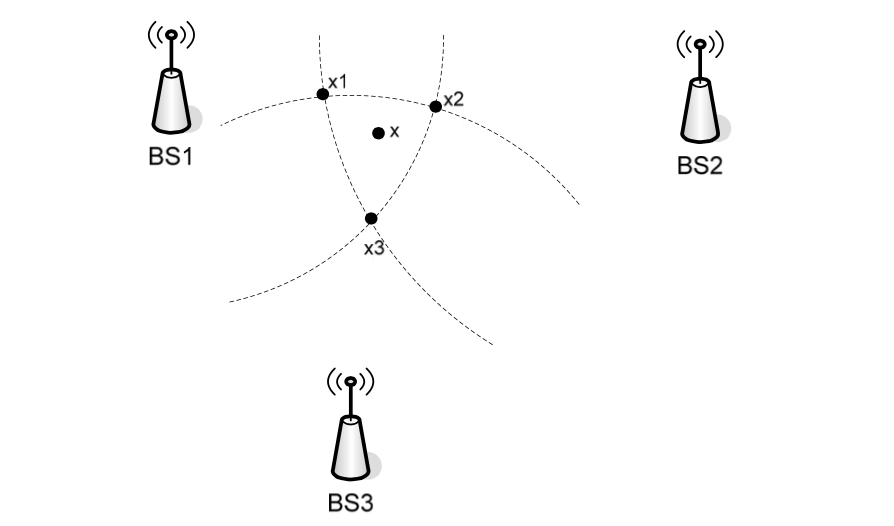
\includegraphics[width=0.45\textwidth]{figures/lateration}
  \label{fig:lateration}
}
\subfloat[Angulation]{
  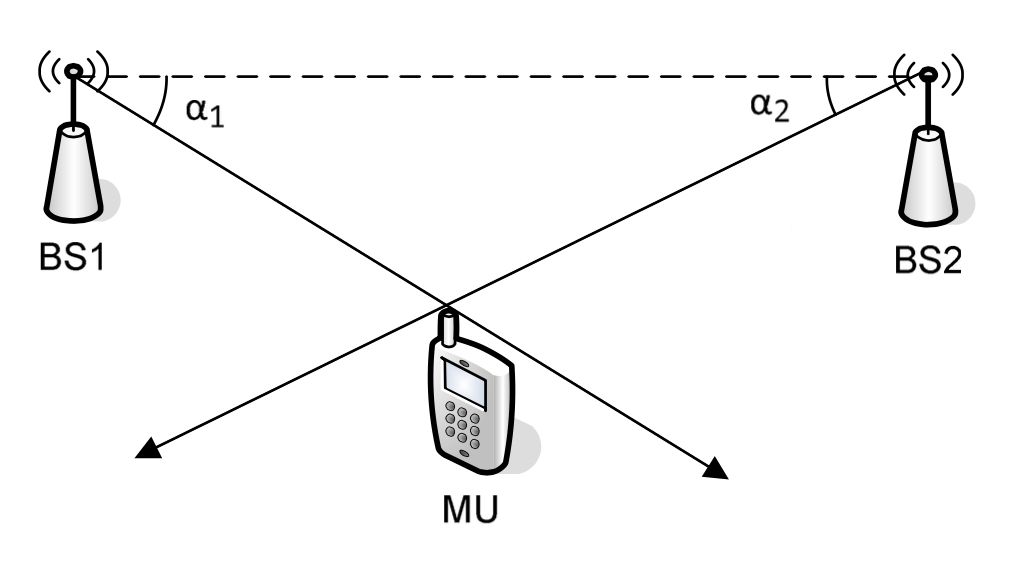
\includegraphics[width=0.45\textwidth]{figures/angulation}
  \label{fig:angulation}
}

	\caption {Principle of the position estimation of a mobile measuring unit using triangulation methods. The wireless signals are transmitted by fixed base stations \citep{wang:bt_pos}.}
	\label{fig:triangulation}
\end{figure}

\subsubsection*{Lateration}
Lateration estimates the location based on the distances from the measuring unit to the transmitters. To precisely estimate a position, three base stations are required. The measuring unit measures the distance to each base station and puts a circle with the radius of the measured distance around the base station. The circles's common intersection point, is the exact position of the mobile unit. In 2D space at least three signals must be received, in 3D, four signals are required. According to \citet{wang:bt_pos}, one common intersection point exists only in theory. In practice, errors, due to obstacles and imperfect propagation models, influence the distances. Thus, no common intersection point exists. Figure~\ref{fig:lateration} depicts this case. Nevertheless, it is possible to estimate the mobile unit's position by using methods such as least-square, three-boarder, or the centroid-method \citep{wang:bt_pos, IEEE:survey_wireless_indoor_pos}.  

The distances for lateration can be estimated by different methods. According to \citet{IEEE:survey_wireless_indoor_pos}, the distance between the measuring unit and the transmitter is directly proportional to the signal's propagation time.
\emph{\ac{TOA}} uses this fact to estimate the distance by measuring the signal's travel time. Consequently, the transmitted signal contains the timestamp of its transmission. Thus, the clocks of all transmitters and measuring units, that are part of the system, need to be precisely synchronized, in order to perform a correct estimation, which is not a trivial problem. For example a timing difference of 1.0~$\mu s$ in a wireless localization system, such as Wifi or \ac{BT}, causes an error of $\approx$~300m, according to \citet{kotanen:exp_local_pos_bt}.

To overcome this disadvantage, a similar method called \emph{\ac{RTOF}} can be used. This method requires all components to be able to receive and transmit signals. The initial transmitter sends a signal, it is received and immediately returned, by the mobile unit. Thus, the transmitter sets the timestamp and compares it with its current timestamp, when the signal arrives. A relative time synchronization is sufficient. But \ac{RTOF} has another problem. The signal is delayed by the processing time, which the unit requires to receive and to send it back to the original source.

The \emph{\ac{TDOA}} method calculates the distance from the different arrival times at the measuring units. Here, the measuring units need to be connected with each other to exchange the timestamps of the signals' arrival and to precisely synchronize their timestamps. The clocks' differences should not exceed tens of nanoseconds \citep{kotanen:exp_local_pos_bt}. The mobile unit, i.e.\ the transmitter, does not need to be synchronized. 

All of the above mentioned methods are based on time, and thus need precisely synchronized or relatively synchronized clocks. According to \citet{IEEE:survey_wireless_indoor_pos}, \ac{TOA} and \ac{TDOA} require a \ac{LOS} channel between transmitter and measuring unit in an indoor environment, because time and angle of the signals' arrival is affected by the multi-path effect, which is a problem of radio propagation. Wireless technologies, such as \acl{BT} and WiFi do have a \emph{\ac{RSSI}} property, which expresses indirectly the signal's \acs{RX}-power level, measured by the device \citep{kotanen:exp_local_pos_bt}. As a consequence, instead of measuring time to calculate the distance between sender and receiver, the loss of the signal strength on its path between the two units can be measured. In order to do that the measuring unit needs to know the initial \ac{RSS} of the emitted signal. As mentioned by \citet{IEEE:survey_wireless_indoor_pos}, different theoretical and empirical models can be used to translate the signals attenuation to a distance estimation, but these models are not always reliable, due to multi-path fading and shadowing in indoor environment.

\subsubsection*{Angulation}
Instead of using distances for the positioning, angulation uses the angles to multiple measurement units, as shown in Figure~\ref{fig:angulation}. In 2D space two angles, in 3D space three angles are sufficient for the positioning. But, to measure the angle of an arriving signal, special directional antennas or arrays of antennas, are required. In the \emph{\ac{AOA}} method, the intersection point of the straights with the measured angles is the mobile units position. Here, highly precise angles need to be measured, which is a big problem in wireless environments due to multi-path reflections and shadowing, as already mentioned before \citep{IEEE:survey_wireless_indoor_pos, wang:bt_pos}.

\subsubsection*{Related Work}
\citet{wang:bt_pos} use Bluetooth to implement an indoor positioning system for mobile devices, like smartphones. The system is based on triangulation methods, i.e.\ on lateration, using \ac{RSS} for the distance estimation. During their research, they evaluate the least-square, three-border, and centroid method for the position estimation. They write, without mentioning any details, that all three methods deliver satisfying results, if the mobile unit receives accurate \ac{RSS} readings and a proper path loss model is used to calculate the distances. They also analyze the effect of placing a human body between transmitter and measuring unit and found out, that the signal is weakened by 6\,--\,8\,dB, which equals a distance of several meters, due to the fact, that decibel~(dB) is a logarithmic unit. Due to the \ac{RSS} values' fluctuation, they propose to filter the \ac{RSS} readings by an average or weighted filter to improve the estimation accuracy.

\citet{oksar:bluetooth} also uses Bluetooth, based on \ac{RSS} readings for indoor localization. In contrast to \citet{wang:bt_pos}, the mobile units are the transmitters, and the measuring units are the fixed base stations with known position. Thus, the system topology is remote positioning. They defined a \emph{root-mean-square-error} function, which compares ``the ratio of the square of distances to the base stations'' with ``the ratio of the signal levels'' \citep{oksar:bluetooth}. The used distances are calculated for assumed discrete positions of the transmitter. As shown by \citet{oksar:bluetooth}, the better the assumed position matches the real position, the smaller is the result of the error function. \citet{oksar:bluetooth} assumes, that the received \ac{RSS} decreases proportional to the squared distance. Thus, compared to \citet{wang:bt_pos}, \citet{oksar:bluetooth} does not directly calculate the distance between the transmitter and the measuring unit. In the mentioned experiment a root-mean-square-error of 2.309\,m of localization accuracy was achieved in the best-case. But \citet{oksar:bluetooth} also mentions, that in a real life application the points are most probably non-discrete points; thus, some changes are necessary.

\citet{hoflinger:acoustic} develop an acoustic indoor localization system called ASSIST, which stands for \emph{Acoustic Self-calibrating System for Indoor Smartphone Tracking}. According to \citet{hoflinger:acoustic}, the system can track a smartphone with an error of 25\,cm. The smartphone sends out a high frequency acoustic signal using its speaker, which is not recognizable for humans. The signal's ``amplitude~A of sound decreases with distance~r according to A\,$\sim$\,1/r''. To detect the signals, fixed measuring units with a sensitive \ac{MEMS} microphone are used. Despite the decreasing amplitude, they can detect the signals in 70\,\% up to 10\,m distance. For the position estimation, the system uses the \ac{TDOA} method. The measuring units are connected via a wired network, which is at the same time the units' power supply. The network is used to synchronize the units' timestamps and to exchange the measured timestamps. According to \citet{hoflinger:acoustic}, also the acoustic signals suffer from echoes and reflections, caused by multi-path propagation. To calculate a robust location, outliers are compensated by using \ac{PF} and \ac{KF}. They also mention, that the system can additionally use inertial smartphone sensors, such as accelerometer, gyroscope, and magnetometer besides the acoustic infrastructure \citep{hoflinger:acoustic, hoflinger:assist}.

Further research projects based on triangulation methods are referenced by \citet{IEEE:survey_wireless_indoor_pos}.


\subsection{Kalman Filter}\label{sec:fund_kf}
The \emph{\acf{KF}}, and the \emph{\acf{EKF}}, are techniques for filtering and prediction of linear and non-linear Gaussian systems with continuous space, such as an indoor robot localization system based on motion and measurements. As mentioned before, localization systems should be able to accommodate for uncertainty. Gaussian filters model the uncertainty of a state~$x$, motion~$u$, and measurement~$z$ as (multivariate) normal distributions. According to \cite{kotanen:exp_local_pos_bt}, with knowing the uncertainties, \ac{KF} optimally minimizes the estimation error's variance.

The algorithm is based on three probabilities. The \emph{state transition probability} $p(x_t | u_t , x_{t-1})$ is the probability for a state~$x_t$, i.e.\ a position, at time~$t$ after the transition from state~$x_{t-1}$ by applying the control i.e.\ motion~$u_t$. The \emph{measurement probability} $p(z_t|x_t)$ defines the probability for a certain measurement~$z_t$ in state~$x_t$, e.g.\ a distance measurement to an obstacle at position~$x_t$. The last probability is the \emph{initial belief}~$bel(x_0)$. It is the probability for the initial state at time t\,=\,0 \citep{thrun:prob_robo}.

The algorithm is iteratively invoked. First it takes the current state and predicts the successive state by applying the motion. Next the measurement based on the predicted state is predicted. Afterwards, the predicted measurement is compared with the real measurement. Based on the comparison's result the algorithm corrects the before predicted state, which is the new state \citep{thrun:prob_robo}.

A detailed description of \ac{KF} and \ac{EKF} is provided by~\citet{thrun:prob_robo}.

\subsubsection*{Related Work}
\ac{KF} can be used for indoor localization by using \acl{BT} technology as demonstrated by \citet{kotanen:exp_local_pos_bt}. They use the signal's \ac{RSS} to estimate the distance between the mobile unit and the transmitters.  Then, they use \ac{EKF} to merge the mobile unit's measurements with the current state, which represents the mobile unit's position in three-dimensional space. Their solution uses a constant state. Thus, no prediction of the successive state by integrating a motion takes place.

As mentioned by \citet{kotanen:exp_local_pos_bt}, the ``main source of errors is unreliability of \ac{RSSI}''. Their position estimation is based on filtered values instead of raw values. But in fact, it relies only on the wireless measurements and does not include additional sensor data or other information, as usual in the robotic's field.  Their solution achieves an absolute positioning error of 3.76\,m.


\subsection{Proximity Method}
The proximity method, which is also known as cell-id tracking, only provides a relative location information. For the localization, the mobile device listens for signals from different transmitters. The transmitters' locations are known and can be identified by their identifier. As a result, the mobile device's location is \emph{next to the transmitter's location} with the strongest signal \citep{IEEE:survey_wireless_indoor_pos, wang:bt_pos}.

As mentioned by \citet{IEEE:survey_wireless_indoor_pos}, the algorithm used by the proximity method is very simple to implement. Additionally, it can use different wireless technologies at the same time, such as Bluetooth, WiFi, etc. The device just needs to \emph{listen} for all of them simultaneously. 

To get a precise position information, many transmitters need to be distributed within the environment. If there are too little, and their range is up to several meters, the location information is very rough \citep{kotanen:exp_local_pos_bt}. As mentioned before, wireless signal's are heavily influenced by the environment. Consequently, it may also happen, that the device's location is not optimal, due to the fact that the signals are not attenuated in the same strength, and thus, the device location is being associated with a transmitter that is further away, than another one.

The solution presented in this thesis follows different approaches. Thus, the proximity method is not explained in more detail. \citet{IEEE:survey_wireless_indoor_pos} gives a more detailed overview of the algorithm and related work.

\subsection{Scene Analysis}\label{sec:fund_sceneanalysis}
Scene analysis localization algorithms, such as \emph{k-Nearest-Neighbors (kNN)}, \emph{Neural Networks}, and \emph{Support Vector Machine (SVM)} are based on machine learning.

According to \citet{IEEE:survey_wireless_indoor_pos}, the use of such algorithms requires two stages, the offline and online stage. During the offline stage, fingerprints are collected at many positions in the area where localization should take place. Most often the fingerprints are \acs{RSS}-based, which means, that at a specific position, the \ac{RSS} values of all received transmitters are collected. Then the fingerprints are stored in a database together with their corresponding location. The online phase is the actual run-time phase, where the localization takes place. To do so, the application creates a fingerprint of the current received signals. Then the algorithm compares the fingerprint with the fingerprints stored in the database during the offline stage and returns the location of the best matching one.

As mentioned by \citet{IEEE:survey_wireless_indoor_pos}, the technique's main challenge is to deal with the signals that are affected by the environment. The scene analysis' offline stage requires a lot of effort, especially in large environments, which is its major disadvantage. Another disadvantage is, that if the environment changes the \ac{RSS} fingerprints can change, too and thus the offline stage needs to be repeated.

The solution presented in this thesis follows different approaches. Thus, scene analysis is not explained in more detail. \citet{IEEE:survey_wireless_indoor_pos} provides a detailed overview of the before mentioned algorithms and related work.
